%%%%%%%%%%%%%%%%%%%%%%%%%%%%%%%%%%%%%%%%%%%%%%%%%%%%%%%%%%%%%%%%%%%%%%%%%%%%%%

\documentclass{l3deliverable}

%%%%%%%%%%%%%%%%%%%%%%%%%%%%%%%%%%%%%%%%%%%%%%%%%%%%%%%%%%%%%%%%%%%%%%%%%%%%%%

\usepackage{graphicx}%
\usepackage{url}%

%%%%%%%%%%%%%%%%%%%%%%%%%%%%%%%%%%%%%%%%%%%%%%%%%%%%%%%%%%%%%%%%%%%%%%%%%%%%%%
%% See D1 for an example of how to integrate sub version revision
%% numbers into a LaTeX document.
%

%%%%%%%%%%%%%%%%%%%%%%%%%%%%%%%%%%%%%%%%%%%%%%%%%%%%%%%%%%%%%%%%%%%%%%%%%%%%%%
%% Check these macro values for appropriateness for your own document.

\title{Draft Submission}

\author{Ross Adam \\
        Andrew Gardner \\
        Nicole Kearns \\
        Mamas Nicolaou\\
	Asset Sarsengaliyev\\}

\date{30th January 2013}

\deliverableID{D6}
\project{PSD3 Group Exercise 2}
\team{V}
\version{0.1}

%%%%%%%%%%%%%%%%%%%%%%%%%%%%%%%%%%%%%%%%%%%%%%%%%%%%%%%%%%%%%%%%%%%%%%%%%%%%%%

\begin{document}

%%%%%%%%%%%%%%%%%%%%%%%%%%%%%%%%%%%%%%%%%%%%%%%%%%%%%%%%%%%%%%%%%%%%%%%%%%%%%%

\maketitle

\tableofcontents

\newpage

%%%%%%%%%%%%%%%%%%%%%%%%%%%%%%%%%%%%%%%%%%%%%%%%%%%%%%%%%%%%%%%%%%%%%%%%%%%%%%
%% Standard section for all documents

\section{Introduction}

\subsection{Identification}
Final report for the internship management project, containing the project plan, requirements specification, a report and demonstration of the prototype.

\subsection{Related Documentation}

PSD3 Group Exercise Description \url{http://fims.moodle.gla.ac.uk/file.php/128/coursework/psd3-ge-1-rev3278.pdf}\\

Deliverables Template \url{http://fims.moodle.gla.ac.uk/file.php/128/coursework/templates.zip}\\

PSD3 Course Notes \url{http://fims.moodle.gla.ac.uk/file.php/128/lecture-notes/notes-r3275.pdf}\\

\subsection{Purpose and Description of Document}
The purpose of this document is to give a detailed description of our
system prototype. This report includes a description of the scope and
design of the system and an evaluation of our prototype.
\subsection{Document Status and Schedule}

\begin{center}{
\begin{tabular}{|c|c|c|c|}
\hline \textbf{Date} &\textbf{ Change} & \textbf{Version} &\textbf{Author}\\ 
\end{tabular} }
\end{center}

%%%%%%%%%%%%%%%%%%%%%%%%%%%%%%%%%%%%%%%%%%%%%%%%%%%%%%%%%%%%%%%%%%%%%%%%%%%%%%

\section{Component Diagram}

%%%%%%%%%%%%%%%%%%%%%%%%%%%%%%%%%%%%%%%%%%%%%%%%%%%%%%%%%%%%%%%%%%%%%%%%%%%%%%

\section{State Diagrams}

\subsection{Rationale}

The following three diagrams were created to illustrate how entities within the application change over time. The three entities are Student, Internship and Advert. These entities were identified by the ``status'' variable in their specification. \\

\subsection{Student}
\textbf{Description} \\

Student was choosen because it displayed 4 distinct states: Approved, Accepted, Withdrawn and Pending. These were identified from the ``View Student Details'' use case. However the finding other use cases to justify this proved difficult as none could be found that implied a change in the Student entity state. Therefore the following diagram was implemented in a manner deemed logical by the team. This is mostly a sub-state diagram encased within a "Not Withdrawn" box. If withdrawn then the sub-state is immediately exited.

\begin{center}
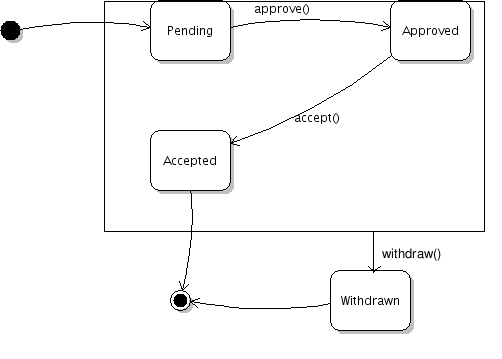
\includegraphics
[scale=0.7]
{img/Student-State.png}
\end{center}

\subsection{Internship}
\textbf{Description}
The Internship has two states Pending and Approved. An Internship starts as either depending on whether it was created by the Course Co-ordinator (Approved) or by a student (Pending). A pending entity can be Approved by the approve method.

\begin{center}
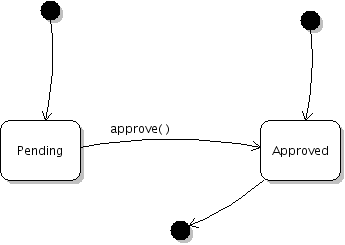
\includegraphics
[scale=0.7]
{img/Internship-state.png}
\end{center}

\subsection{Advert}
\textbf{Description}
An Advert can have the following states: Pendign, Not Published and Published. An advert always starts in the pending state, from there it can either become Not Published or Published. It becomes Published if it is deemed acceptable by the Course Co-ordinator and it becomes Not Published if it needs revised. Only a pending or Not Published article can be revised.

\begin{center}
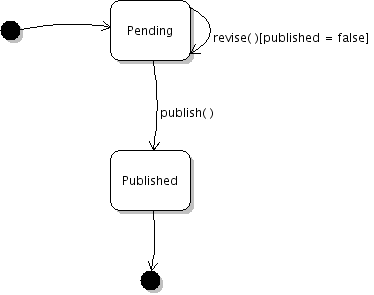
\includegraphics
[scale=0.7]
{img/Advert-State.png}
\end{center}

%%%%%%%%%%%%%%%%%%%%%%%%%%%%%%%%%%%%%%%%%%%%%%%%%%%%%%%%%%%%%%%%%%%%%%%%%%%%%%

\section{Class Diagrams}

%%%%%%%%%%%%%%%%%%%%%%%%%%%%%%%%%%%%%%%%%%%%%%%%%%%%%%%%%%%%%%%%%%%%%%%%%%%%%%

\section{API Specification}


\subsection{Advert Store}

\textbf{Method}: Public Advert getAdvert(integer advertId)\\
\textbf{Description}: Gets the advert with the given advert id.\\
\textbf{Parameters}: integer advertId\\
\textbf{Return Type}: Advert\\
\textbf{Pre Condition}: Advert with the given id is available within the system. \\
\textbf{Post Condition}: \\

\textbf{Method}:Public void removeAdvert(integer advertId)\\
\textbf{Description}: The advert with the given advert id is no longer available and removed from the system.\\
\textbf{Parameters}: Integer advertId\\
\textbf{Return Type}: \\
\textbf{Pre Condition}: Advert with the given id is available within the system.\\
\textbf{Post Condition}: Advert is no longer available on the system.\\

\textbf{Method}: Public Boolean advertExists(integer advertId)\\
\textbf{Description}: Checks if a specific advert does exist in the advert store.\\
\textbf{Parameters}: Integer advertId\\
\textbf{Return Type}: Boolean\\
\textbf{Pre Condition}:\\
\textbf{Post Condition}:\\

\textbf{Method}: Public void storeAdvert(integer advertId)\\
\textbf{Description}: Adds a new advert with the given advert id to the advert store. \\
\textbf{Parameters}: Integer advertId\\
\textbf{Return Type}: \\
\textbf{Pre Condition}: Advert is not already stored in the advert store.\\
\textbf{Post Condition}: Advert is now stored in the advert store.\\

\subsection{Offer Store}

\textbf{Method}: Public Offer getOffer(integer offerId)\\ 
\textbf{Description}: Gets the offer with the given offer id. \\
\textbf{Parameters}: Integer offerId\\
\textbf{Return Type}: Offer\\
\textbf{Pre Condition}: Offer with given id is stored in the system.\\
\textbf{Post Condition}:\\

\textbf{Method}: Public void removeOffer(integer offerId)\\
\textbf{Description}: The offer with the given offer id is removed from the system. \\
\textbf{Parameters}: Integer offerId \\
\textbf{Return Type}:\\
\textbf{Pre Condition}: offer with the given id is available within the system.\\
\textbf{Post Condition}: offer is no longer stored on the system.\\

\textbf{Method}: Public Boolean offerExists(integer offerId) \\
\textbf{Description}: Checks if a specific offer is stored within the offer store. \\
\textbf{Parameters}: Integer offerId\\
\textbf{Return Type}: Boolean\\
\textbf{Pre Condition}:\\
\textbf{Post Condition}:\\

\textbf{Method}: Public void storeOffer(integer offerId)\\
\textbf{Description}: Adds a new offer with the given offer id to the offer store. \\
\textbf{Parameters}: Integer offerId\\
\textbf{Return Type}:\\
\textbf{Pre Condition}: offer is not already stored in the offer store.\\
\textbf{Pre Condition}: student notifies course coordinator of internship placement offer.\\
\textbf{Post Condition}: offer is now stored in the offer store.\\

\subsection{Visit Store}

\textbf{Method}: Public Visit getVisit(integer visitId)\\
\textbf{Description}: Gets the visit with the given visit id. \\
\textbf{Parameters}: Integer visitId\\
\textbf{Return Type}: Visit\\
\textbf{Pre Condition}: Visit details are stored in the system.\\
\textbf{Post Condition}:\\

\textbf{Method}: Public void removeVisit(integer advertId)\\
\textbf{Description}: The visit details with the given visit id removed from the system. \\
\textbf{Parameters}: Integer visitId\\
\textbf{Return Type}:\\
\textbf{Pre Condition}: visit details with the given id are available within the system.\\
\textbf{Post Condition}: visit details are no longer available on the system.\\

\textbf{Method}: Public Boolean visitExists(integer adverted)\\
\textbf{Description}: Checks if a specific visit does is stored in the visit store. \\
\textbf{Parameters}: Integer visitId\\
\textbf{Return Type}: Boolean\\
\textbf{Pre Condition}:\\
\textbf{Post Condition}:\\

\textbf{Method}: Public void storeVisit(integer visitId) \\
\textbf{Description}:  adds the details of a new visit with the given visit id to the visit store.\\
\textbf{Parameters}: Integer visitId\\
\textbf{Return Type}:\\
\textbf{Pre Condition}: Visit is not already stored in the visit store.\\
\textbf{Post Condition}: visit is now stored in the visit store.\\

\subsection{Employer Store}

\textbf{Method}: Public Employer getEmployer(integer employerId)\\
\textbf{Description}: Gets the employer with the given employer id.\\
\textbf{Parameters}:  Integer employerId\\
\textbf{Return Type}: Employer\\
\textbf{Pre Condition}: Employer with given employerId is available in the system.\\
\textbf{Post Condition}:\\

\textbf{Method}: Public void removeEmployer(integer employerId) \\
\textbf{Description}: will remove the employer with the specified id from the system, meaning that they can no longer log in to the system\\
\textbf{Parameters}: Integer empoyerId\\
\textbf{Return Type}:\\
\textbf{Pre Condition}: The employer is stored in the Employer Store\\
\textbf{Post Condition}: The employer details are no longer available/stored.\\

\textbf{Method}: Public boolean employerExists(integer employerId) \\
\textbf{Description}: checks if a specific employer is stored within the employer store.\\
\textbf{Parameters}: Integer employerId\\
\textbf{Return Type}: Boolean\\
\textbf{Pre Condition}:\\
\textbf{Post Condition}:\\

\textbf{Method}: Public void storeEmployer(integer employerId) \\
\textbf{Description}:  Adds a new Employer with the given Employer id to the Employer store.\\
\textbf{Parameters}: Integer employerId\\
\textbf{Return Type}:\\
\textbf{Pre Condition}: employer with the specified id does not exist in the employer store.\\
\textbf{Post Condition}: Employer is stored in the employer store.\\

\textbf{Method}: Public void setEmployerPassword(String password) \\
\textbf{Description}: Allows the Employer to set up a new password.\\
\textbf{Parameters}: String password\\
\textbf{Return Type}: \\
\textbf{Pre Condition}: Employer with given id is available in the system.\\
\textbf{Post Condition}: New password is now set to the String passed in.\\

\textbf{Method}: Public String getEmployerPassword() \\
\textbf{Description}: Will provide the user with the password for the specific employer.\\
\textbf{Parameters}:\\
\textbf{Return Type}: String \\
\textbf{Pre Condition}: Employer is available in the system.\\
\textbf{Post Condition}:\\

\textbf{Method}: Public String getEmployerName()\\
\textbf{Description}: Gets the name of the employer with a specific employer id.\\
\textbf{Parameters}:\\
\textbf{Return Type}: String\\
\textbf{Pre Condition}: Employer with given id is available in the system.\\
\textbf{Post Condition}:\\

\textbf{Method}: Public void setEmployerName(String name)\\
\textbf{Description}: Allows the user to set the name of the employer for the specified employer.\\
\textbf{Parameters}: String name\\
\textbf{Return Type}:\\
\textbf{Pre Condition}: Employer with given id is available in the system.\\
\textbf{Post Condition}: Employer name is now set to the String given.\\

\textbf{Method}: Public void getEmployerEmail()\\
\textbf{Description}: Gets the email address for the employer with a specific employer id.\\
\textbf{Parameters}:\\
\textbf{Return Type}:\\
\textbf{Pre Condition}: Employer with given id is available in the system.\\
\textbf{Post Condition}:\\

\textbf{Method}: Public void setEmployerEmail(String email)\\
\textbf{Description}: Allows the user to set the email address of the employer for the specified employer.\\
\textbf{Parameters}:String email\\
\textbf{Return Type}:\\
\textbf{Pre Condition}: Employer with given id is available in the system.\\
\textbf{Post Condition}: The email address of the employer is set to the String provided.\\

\subsection{GU User Store}

\textbf{Method}: Public GUuser getGUuser(integer GUuserId)\\
\textbf{Description}: Gets the employer with the given GUID.\\
\textbf{Parameters}: Integer GUuserId\\
\textbf{Return Type}: GUuser\\
\textbf{Pre Condition}: GUuser with given GUuserId is available in the system.\\
\textbf{Post Condition}:\\

\textbf{Method}: Public void removeGUuser(integer GuuserId)\\
\textbf{Description}: Will remove the GU user with the specified id from the system, meaning that they can no longer log in to the system.
\\
\textbf{Parameters}: Integer GUuserId\\
\textbf{Return Type}:\\
\textbf{Pre Condition}: GU user details are stored in the GU user store\\
\textbf{Post Condition}: User details are no longer available in the GU user store\\

\textbf{Method}: Public boolean GUuserExists(integer GuuserId)\\
\textbf{Description}: Checks if a specific GU user is stored within the GU user store.\\
\textbf{Parameters}: Integer GUuserId\\
\textbf{Return Type}: Boolean\\
\textbf{Pre Condition}:\\
\textbf{Post Condition}:\\

\textbf{Method}: Public void storeGUuser (integer GUuserId)\\
\textbf{Description}: Adds a new GU user with the given GUuser id to the GU user store.\\
\textbf{Parameters}: Integer GUuserId\\
\textbf{Return Type}:\\
\textbf{Pre Condition}: No user with the given id is stored in the GU user store\\
\textbf{Post Condition}: GU user is stored in the GU user store.\\

\textbf{Method}: Public String getGUuserName()\\
\textbf{Description}: Gets the name of the GU user with a specific GU user id.\\
\textbf{Parameters}:\\
\textbf{Return Type}: String\\
\textbf{Pre Condition}: GU user with given id is stored in the system.\\
\textbf{Post Condition}:\\

\textbf{Method}: Public void setGUuserName(String name)\\
\textbf{Description}: Allows the user to set the name of the GU user for the specified GUuser Id.\\
\textbf{Parameters}: String name\\
\textbf{Return Type}:\\
\textbf{Pre Condition}: GU user is stored in the system.\\
\textbf{Post Condition}: The name of the GU user is set to the String provided.\\

\textbf{Method}: Public void getGUuserEmail(Integer GUuserId)\\
\textbf{Description}: Gets the email address for the GU user with a specific GUuser id.\\
\textbf{Parameters}: Integer GUuserId\\
\textbf{Return Type}:\\
\textbf{Pre Condition}: GUuser with the given id is available within the system.\\
\textbf{Post Condition}:\\

\subsection{Employer Authentication}

\textbf{Method}: Public void authenticateEmpUser(String username, String password)\\
\textbf{Description}: Checks that the username and password for the user are correct.\\
\textbf{Parameters}: String username, String password\\
\textbf{Return Type}:\\
\textbf{Pre Condition}: Employer user is not logged in to the system.\\
\textbf{Post Condition}: Employer is logged into the system.\\

\subsection{GU User Authentication}

\textbf{Method}: Public void authenticateGUuser(String username, String password)\\
\textbf{Description}: Checks that the username and password for the user are correct. \\
\textbf{Parameters}: String username, String password\\
\textbf{Return Type}:\\
\textbf{Pre Condition}: GU user is not logged in to the system.\\
\textbf{Post Condition}: GU user is logged into the system.\\

%%%%%%%%%%%%%%%%%%%%%%%%%%%%%%%%%%%%%%%%%%%%%%%%%%%%%%%%%%%%%%%%%%%%%%%%%%%%%%

\section{Acceptance Tests}

\end{document}
